\section{Measurement of Market Efficiency}
\label{sec:market_efficiency}

In this section, we will introduce the $Beta\_SSE$ score, which is a measure of market efficiency based on the unbiasedness regressions framework.

\subsection{Unbiasedness Regressions}

\noindent The unbiasedness regression is a simple OLS regression of the cumulative logarithmic return of the asset over a normalized window of time $\mathrm{SP500}_{[0, T]}$, on a subset of the
logarithmic cumulative returns, $\mathrm{SP500}_{[0, t]}$, where $t \leq T$, and $t$ is the number of months from the beginning of the window.
 \footnote{$\mathrm{SP500}_{[0, 1]}$ is the matrix of returns of the SP500 from January 1950 to February 1950, February 1950 to March 1950, \dots, August 2024 to September 2024, September 2024 to October 2024.\newline
$\mathrm{SP500}_{[0, 2]}$ would be the matrix of cumulative returns from January 1950 to March 1950, February 1950 to April 1950, \dots August 2024 to October 2024, and so on for the entire dataset.}

\begin{equation}
    \begin{aligned}
        \mathrm{SP500}_{[0, T]} &= \alpha_t + \beta_t \mathrm{SP500}_{[0, t]} + \epsilon_{t}, \hfill \text{   where } 0 \leq t \leq T.
    \end{aligned}
\end{equation}

\noindent For an illustrative example, let $T = 36$, so that the window $[0, T]$ represents a 3-year period, and let us look at the returns of the SP500.

\noindent For $t=1$, the regression is of the form:
\begin{equation}
    \mathrm{SP500}_{[0, 36]} = \alpha + \beta \mathrm{SP500}_{[0, 1]} + \epsilon
\end{equation}

\noindent From this regression we extract the coefficient $\beta$ and the $R^2$ value.
The regression is repeated for $t=2, t=3, ..., t=36$, and the coefficients $\beta$ as well as the $R^2$ are plotted against $t$.

\begin{figure}[h!]
    \centering
    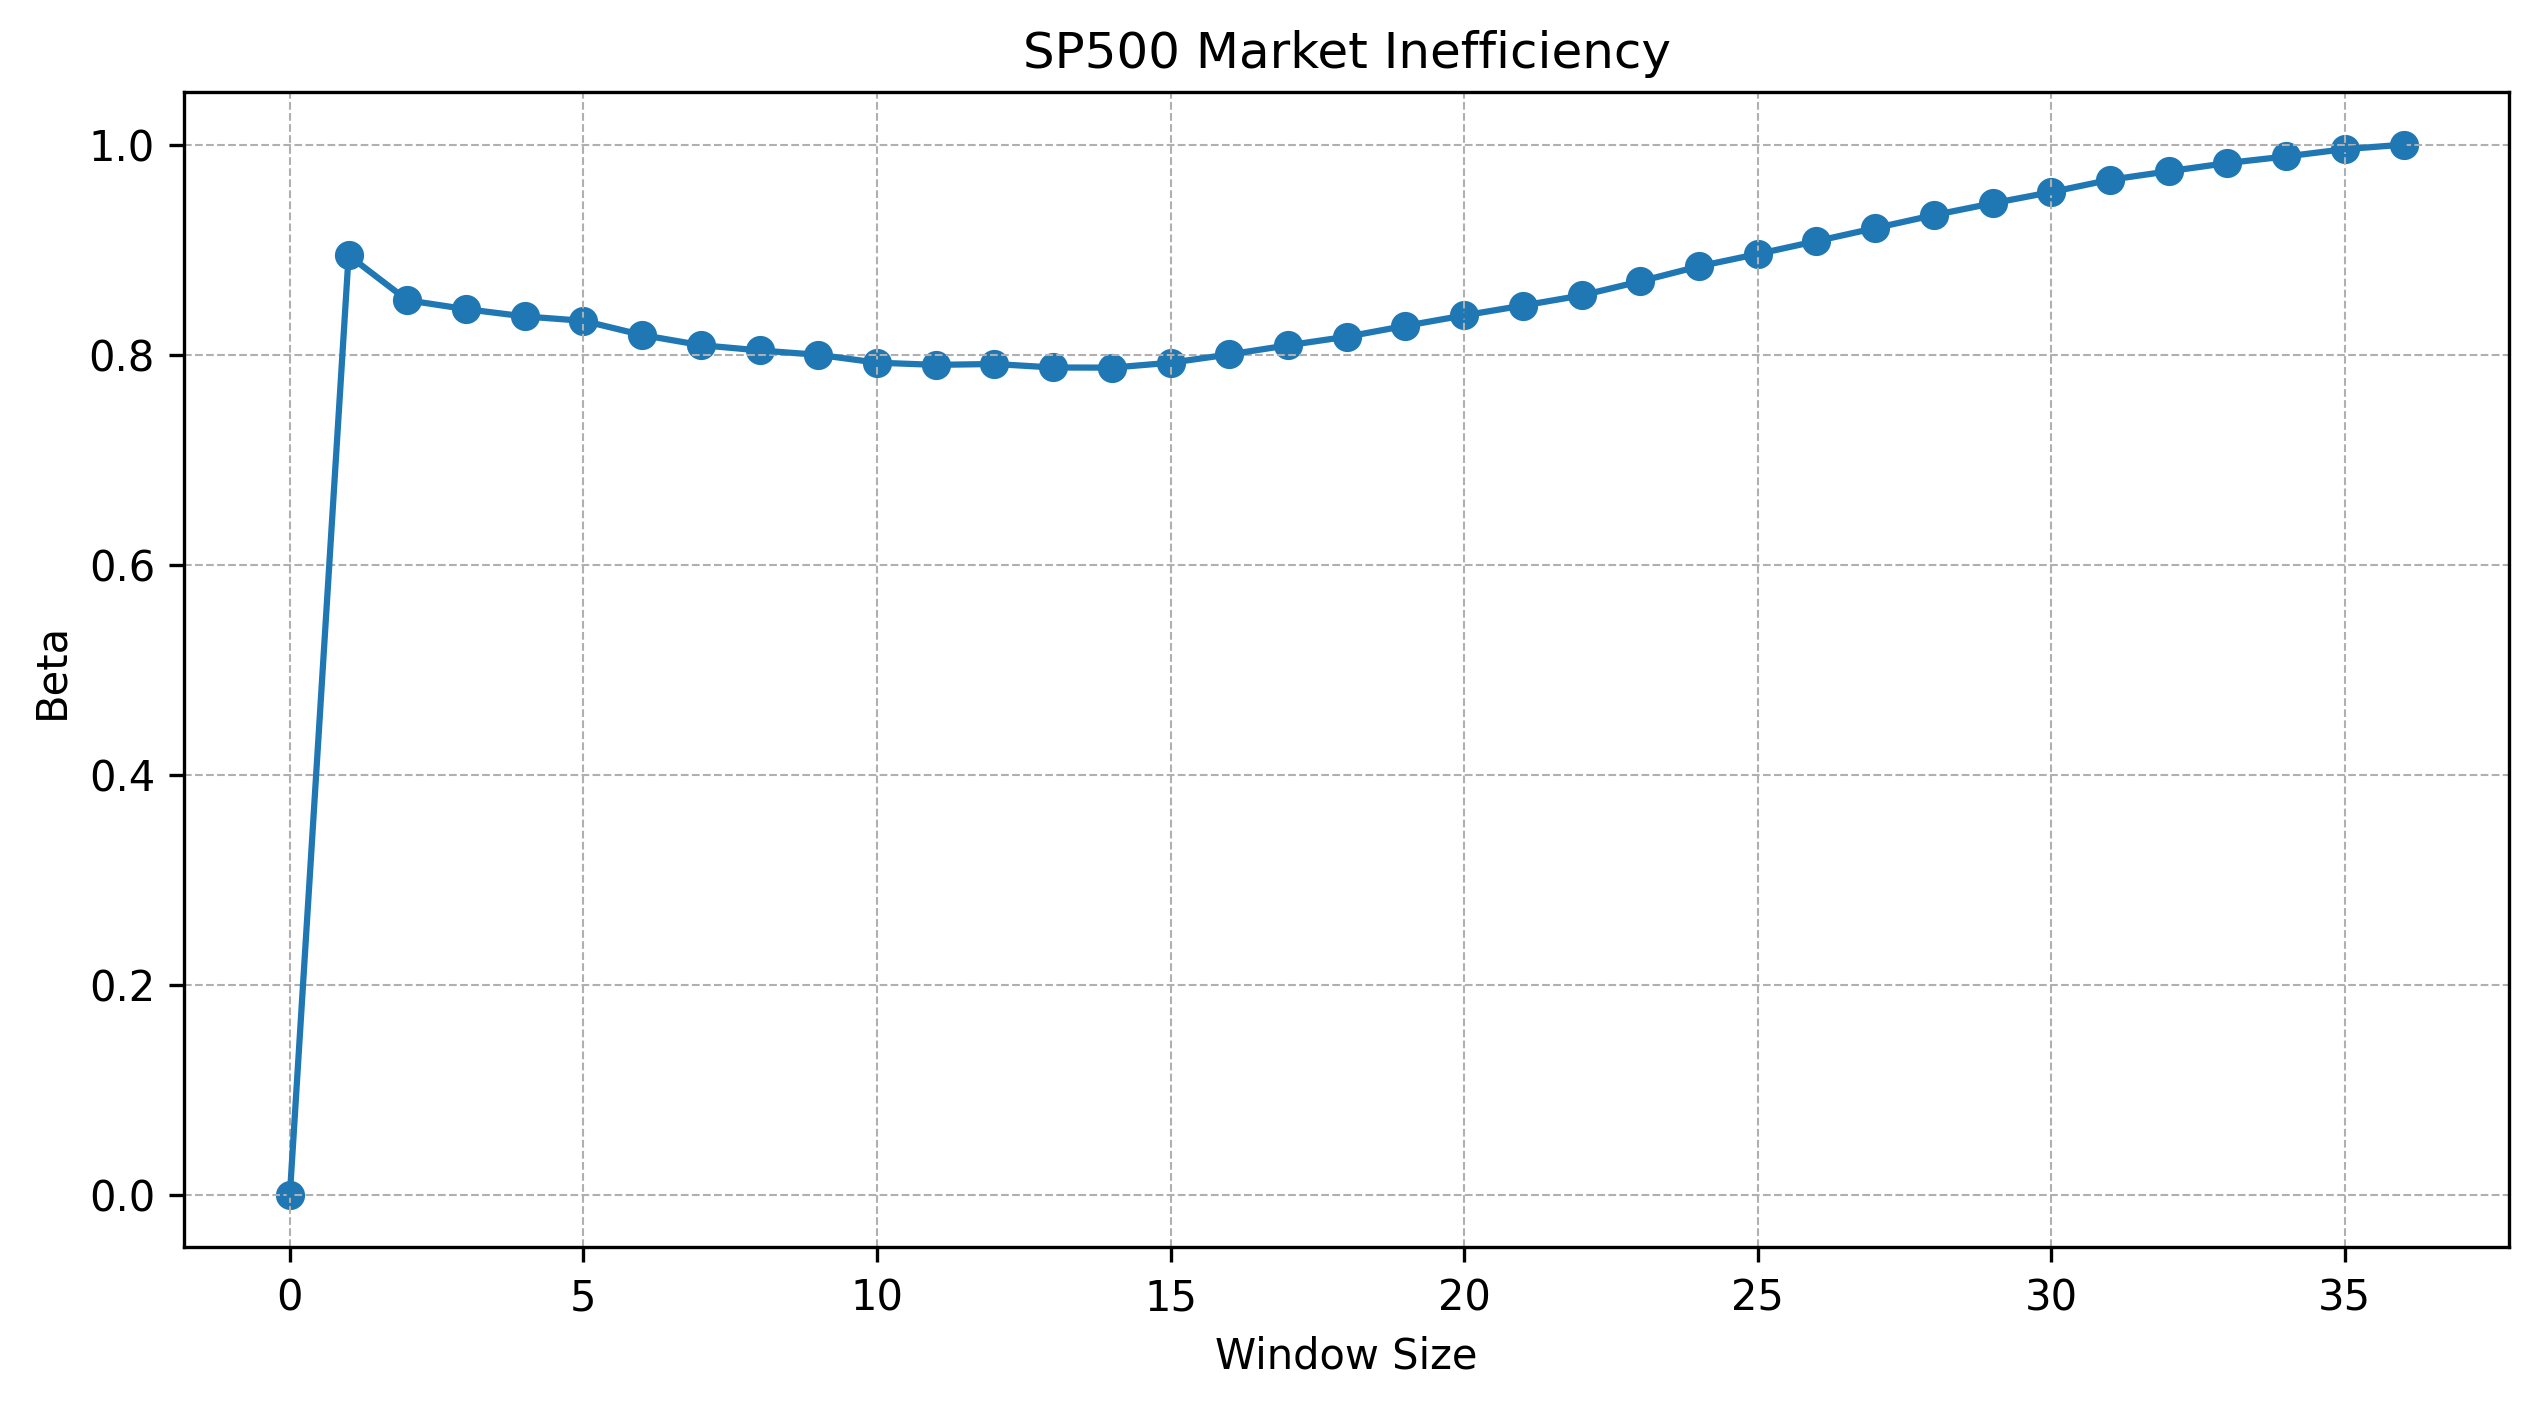
\includegraphics[width=0.8\textwidth]{../figs/SP500 Market Inefficiency.png}
    \caption{An example of an unbiasedness regression on the SP500 (1950 - 2024)}
    \label{fig:sp_500_unbiasedness}
\end{figure}

% THIS IS COPIED FROM CHARLES CHANGE THIS IN DRAFT UPDATE
When log prices form a random-walk with drift, as in efficient markets, $\beta_t = 1$ for all $t$. 
As per \citet{mincer_zarnowitz_1969}, when $\beta_t = 1$, the partial return from $0$ to $t$ provides an "efficient" forecast of the return
from $t$ to $T$. 2, in the sense that no amplification or attenuation of the partial return can improve the residual variance
of the forecast error. If $\beta_t < 1$, then the partial return is attenuated or partially reversed in the total return, which is often interpreted as a symptom of price noise,
a temporary component in prices, or “overreaction” \citep{barclay_hendershott_2003}. Conversely, if $\beta_t > 1$, the partial return is amplified in the total return, suggesting “underreaction” or slow information processing.
% THIS IS COPIED FROM CHARLES CHANGE THIS IN DRAFT UPDATE

In this paper we will be focusing on the $\beta_t$ coefficient, but an explanation of the $R^2$ is provided in the Appendix for completeness. 
We now have the foundation to construct a score for market efficiency.

\subsection{$Beta\_SSE$ Score}

We have established the unbiasedness regression infrastructure, and that a $\beta_t < 1$ indicates overreaction, a $\beta_t > 1$ indicates underreaction, and $\beta_t = 1$ indicates efficiency.
To construct a score that measures the level of market efficiency at a point in time, we have to create a representation of the $\beta_t$ graph for a time period.

We define the $Beta\_SSE$ score as the sum of the squared differences between $\beta_t$ and the horizontal line at $\beta = 1$, for all $t$ in the window.
Since a $\beta_t = 1$ indicates efficiency, the $Beta\_SSE$ score will be lower when the market is more efficient and larger when the market is less efficient, whether by under- or over-reaction.

To construct a timeseries of these scores, we run the unbiasedness regressions on a rolling window of five years.
So $Beta\_SSE_t$ is constructed from the unbiasedness regressions of the SP500 where $t=0$ in the regression are the month beginnings in the period
$t - 5 \times 12$ to $t$.
\footnote{Note that our unbiasedness regressions exted out to $t+36$, so $Beta\_SSE_t$ score isn't tradeable at time $t$ but at time $t+36$. Consider the window [January 2000, January 2005], the observation starting at January 2005 requires the window of returns from January 2005 to January 2008 to make $\mathrm{SP500}_{[0, 36]}$.}

\begin{equation}
    \begin{aligned}
        Beta\_SSE_t &= \sum_{i=0}^{36} (\beta_{t,i} - 1)^2
    \end{aligned}
\end{equation}

Where $\beta_{t,i}$ is the $\beta$ coefficient from the unbiasedness regression from a 
window ending on the date $t$, at the $i$th depth of the unbiasedness window.
